\documentclass{standalone}
\usepackage{tikz}
\usetikzlibrary{patterns, positioning}


\begin{document}
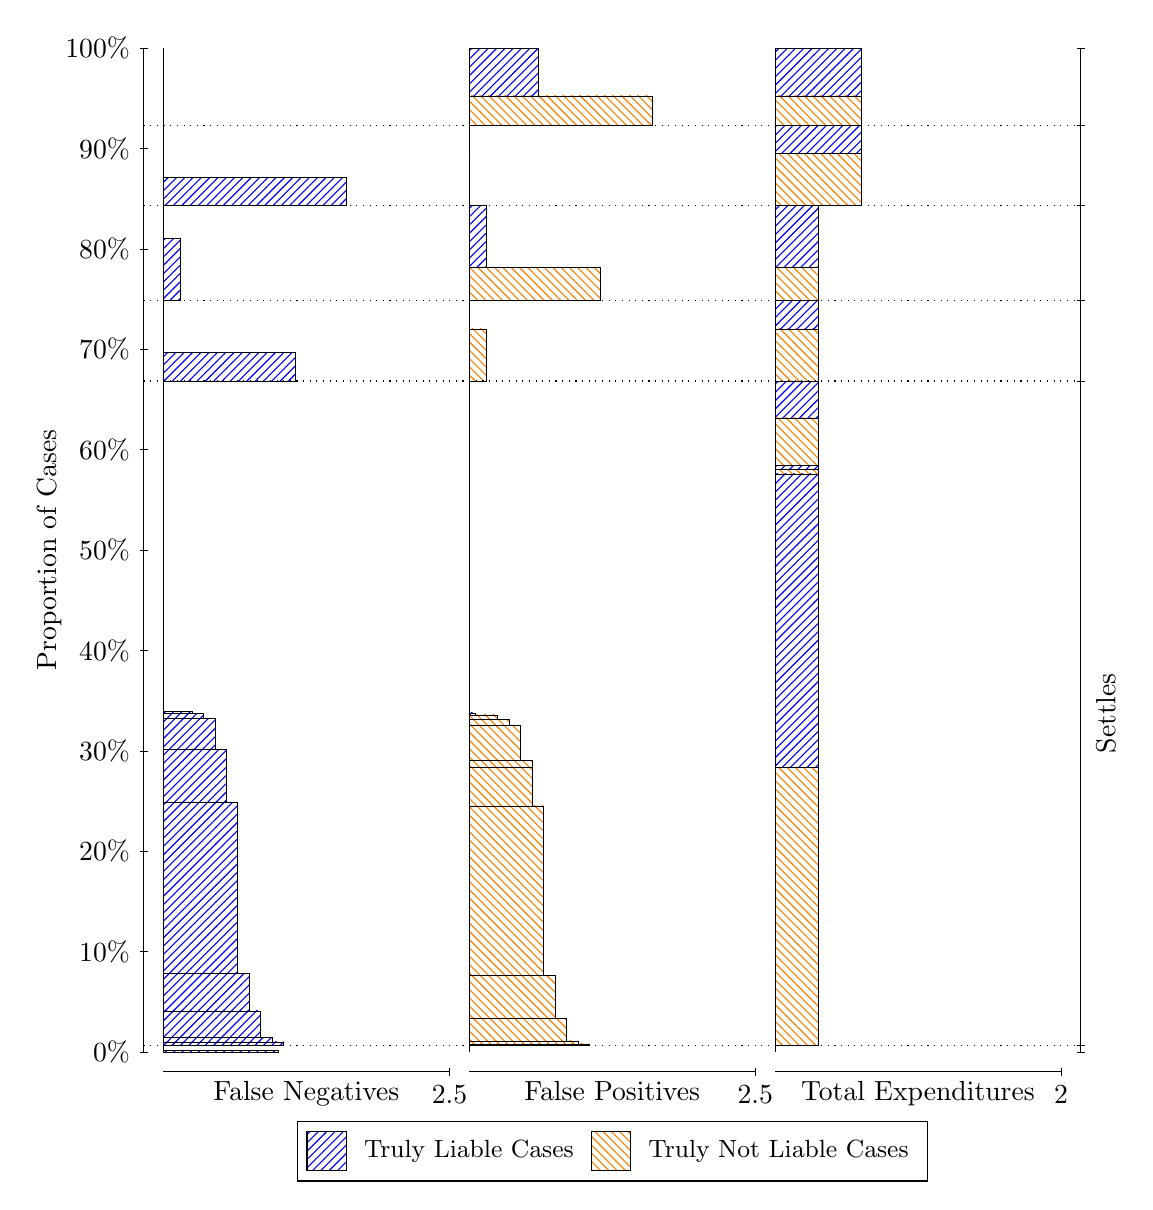
\begin{tikzpicture}
\draw[black, very thin] (1.5,1.75) -- (1.5,14.5);
\node[rotate=90, text=black, anchor=center] at (0.3, 8.125) {Proportion of Cases};
\draw[black, very thin] (1.45,1.75) -- (1.55,1.75);
\node[text=black, anchor=east] at (1.45, 1.75) {0\%};
\draw[black, very thin] (1.45,3.025) -- (1.55,3.025);
\node[text=black, anchor=east] at (1.45, 3.025) {10\%};
\draw[black, very thin] (1.45,4.3) -- (1.55,4.3);
\node[text=black, anchor=east] at (1.45, 4.3) {20\%};
\draw[black, very thin] (1.45,5.575) -- (1.55,5.575);
\node[text=black, anchor=east] at (1.45, 5.575) {30\%};
\draw[black, very thin] (1.45,6.85) -- (1.55,6.85);
\node[text=black, anchor=east] at (1.45, 6.85) {40\%};
\draw[black, very thin] (1.45,8.125) -- (1.55,8.125);
\node[text=black, anchor=east] at (1.45, 8.125) {50\%};
\draw[black, very thin] (1.45,9.4) -- (1.55,9.4);
\node[text=black, anchor=east] at (1.45, 9.4) {60\%};
\draw[black, very thin] (1.45,10.675) -- (1.55,10.675);
\node[text=black, anchor=east] at (1.45, 10.675) {70\%};
\draw[black, very thin] (1.45,11.95) -- (1.55,11.95);
\node[text=black, anchor=east] at (1.45, 11.95) {80\%};
\draw[black, very thin] (1.45,13.225) -- (1.55,13.225);
\node[text=black, anchor=east] at (1.45, 13.225) {90\%};
\draw[black, very thin] (1.45,14.5) -- (1.55,14.5);
\node[text=black, anchor=east] at (1.45, 14.5) {100\%};

\draw[black, very thin] (13.4,1.75) -- (13.4,14.5);
\draw[black, very thin] (13.35,1.75) -- (13.45,1.75);
\node[anchor=west] at (13.35, 1.75) {};
\draw[black, very thin] (13.35,1.8339) -- (13.45,1.8339);
\node[anchor=west] at (13.35, 1.8339) {};
\draw[black, very thin] (13.35,10.271) -- (13.45,10.271);
\node[anchor=west] at (13.35, 10.271) {};
\draw[black, very thin] (13.35,11.298) -- (13.45,11.298);
\node[anchor=west] at (13.35, 11.298) {};
\draw[black, very thin] (13.35,12.498) -- (13.45,12.498);
\node[anchor=west] at (13.35, 12.498) {};
\draw[black, very thin] (13.35,13.518) -- (13.45,13.518);
\node[anchor=west] at (13.35, 13.518) {};
\draw[black, very thin] (13.35,14.5) -- (13.45,14.5);
\node[anchor=west] at (13.35, 14.5) {};

\draw[black, very thin, pattern color=blue, pattern=north east lines] (1.75,1.75) rectangle (3.2033,1.773);
\draw[black, very thin, pattern color=orange, pattern=north west lines] (1.75,1.773) rectangle (1.75,1.8339);
\draw[black, very thin, pattern color=blue, pattern=north east lines] (1.75,1.8339) rectangle (3.276,1.8788);
\draw[black, very thin, pattern color=blue, pattern=north east lines] (1.75,1.8788) rectangle (3.1307,1.9357);
\draw[black, very thin, pattern color=blue, pattern=north east lines] (1.75,1.9357) rectangle (2.9853,2.2727);
\draw[black, very thin, pattern color=blue, pattern=north east lines] (1.75,2.2727) rectangle (2.84,2.7443);
\draw[black, very thin, pattern color=blue, pattern=north east lines] (1.75,2.7443) rectangle (2.6947,4.9226);
\draw[black, very thin, pattern color=blue, pattern=north east lines] (1.75,4.9226) rectangle (2.5493,5.5901);
\draw[black, very thin, pattern color=blue, pattern=north east lines] (1.75,5.5901) rectangle (2.404,5.9876);
\draw[black, very thin, pattern color=blue, pattern=north east lines] (1.75,5.9876) rectangle (2.2587,6.0494);
\draw[black, very thin, pattern color=blue, pattern=north east lines] (1.75,6.0494) rectangle (2.1133,6.074);
\draw[black, very thin, pattern color=orange, pattern=north west lines] (1.75,6.074) rectangle (1.75,10.271);
\draw[black, very thin, pattern color=blue, pattern=north east lines] (1.75,10.271) rectangle (3.4213,10.636);
\draw[black, very thin, pattern color=orange, pattern=north west lines] (1.75,10.636) rectangle (1.75,11.298);
\draw[black, very thin, pattern color=blue, pattern=north east lines] (1.75,11.298) rectangle (1.968,12.081);
\draw[black, very thin, pattern color=orange, pattern=north west lines] (1.75,12.081) rectangle (1.75,12.498);
\draw[black, very thin, pattern color=blue, pattern=north east lines] (1.75,12.498) rectangle (4.0753,12.854);
\draw[black, very thin, pattern color=orange, pattern=north west lines] (1.75,12.854) rectangle (1.75,13.518);
\draw[black, very thin, pattern color=orange, pattern=north west lines] (1.75,13.518) rectangle (1.75,13.891);
\draw[black, very thin, pattern color=blue, pattern=north east lines] (1.75,13.891) rectangle (1.75,14.5);
\draw[black, very thin, pattern color=orange, pattern=north west lines] (5.6333,1.75) rectangle (5.6333,1.8109);
\draw[black, very thin, pattern color=blue, pattern=north east lines] (5.6333,1.8109) rectangle (5.6333,1.8339);
\draw[black, very thin, pattern color=orange, pattern=north west lines] (5.6333,1.8339) rectangle (7.1593,1.8528);
\draw[black, very thin, pattern color=orange, pattern=north west lines] (5.6333,1.8528) rectangle (7.014,1.8922);
\draw[black, very thin, pattern color=orange, pattern=north west lines] (5.6333,1.8922) rectangle (6.8687,2.1778);
\draw[black, very thin, pattern color=orange, pattern=north west lines] (5.6333,2.1778) rectangle (6.7233,2.7204);
\draw[black, very thin, pattern color=orange, pattern=north west lines] (5.6333,2.7204) rectangle (6.578,4.8749);
\draw[black, very thin, pattern color=orange, pattern=north west lines] (5.6333,4.8749) rectangle (6.4327,5.3647);
\draw[black, very thin, pattern color=orange, pattern=north west lines] (5.6333,5.3647) rectangle (6.4327,5.4532);
\draw[black, very thin, pattern color=orange, pattern=north west lines] (5.6333,5.4532) rectangle (6.2873,5.9017);
\draw[black, very thin, pattern color=orange, pattern=north west lines] (5.6333,5.9017) rectangle (6.142,5.9703);
\draw[black, very thin, pattern color=orange, pattern=north west lines] (5.6333,5.9703) rectangle (5.9967,6.0311);
\draw[black, very thin, pattern color=blue, pattern=north east lines] (5.6333,6.0311) rectangle (5.706,6.0558);
\draw[black, very thin, pattern color=blue, pattern=north east lines] (5.6333,6.0558) rectangle (5.6333,10.271);
\draw[black, very thin, pattern color=orange, pattern=north west lines] (5.6333,10.271) rectangle (5.8513,10.934);
\draw[black, very thin, pattern color=blue, pattern=north east lines] (5.6333,10.934) rectangle (5.6333,11.298);
\draw[black, very thin, pattern color=orange, pattern=north west lines] (5.6333,11.298) rectangle (7.3047,11.716);
\draw[black, very thin, pattern color=blue, pattern=north east lines] (5.6333,11.716) rectangle (5.8513,12.498);
\draw[black, very thin, pattern color=orange, pattern=north west lines] (5.6333,12.498) rectangle (5.6333,13.162);
\draw[black, very thin, pattern color=blue, pattern=north east lines] (5.6333,13.162) rectangle (5.6333,13.518);
\draw[black, very thin, pattern color=orange, pattern=north west lines] (5.6333,13.518) rectangle (7.9587,13.891);
\draw[black, very thin, pattern color=blue, pattern=north east lines] (5.6333,13.891) rectangle (6.5053,14.5);
\draw[black, very thin, pattern color=orange, pattern=north west lines] (9.5167,1.75) rectangle (9.5167,1.8109);
\draw[black, very thin, pattern color=blue, pattern=north east lines] (9.5167,1.8109) rectangle (9.5167,1.8339);
\draw[black, very thin, pattern color=orange, pattern=north west lines] (9.5167,1.8339) rectangle (10.062,5.3647);
\draw[black, very thin, pattern color=blue, pattern=north east lines] (9.5167,5.3647) rectangle (10.062,9.0929);
\draw[black, very thin, pattern color=orange, pattern=north west lines] (9.5167,9.0929) rectangle (10.062,9.1537);
\draw[black, very thin, pattern color=blue, pattern=north east lines] (9.5167,9.1537) rectangle (10.062,9.1986);
\draw[black, very thin, pattern color=orange, pattern=north west lines] (9.5167,9.1986) rectangle (10.062,9.8042);
\draw[black, very thin, pattern color=blue, pattern=north east lines] (9.5167,9.8042) rectangle (10.062,10.271);
\draw[black, very thin, pattern color=orange, pattern=north west lines] (9.5167,10.271) rectangle (10.062,10.934);
\draw[black, very thin, pattern color=blue, pattern=north east lines] (9.5167,10.934) rectangle (10.062,11.298);
\draw[black, very thin, pattern color=orange, pattern=north west lines] (9.5167,11.298) rectangle (10.062,11.716);
\draw[black, very thin, pattern color=blue, pattern=north east lines] (9.5167,11.716) rectangle (10.062,12.498);
\draw[black, very thin, pattern color=orange, pattern=north west lines] (9.5167,12.498) rectangle (10.607,13.162);
\draw[black, very thin, pattern color=blue, pattern=north east lines] (9.5167,13.162) rectangle (10.607,13.518);
\draw[black, very thin, pattern color=orange, pattern=north west lines] (9.5167,13.518) rectangle (10.607,13.891);
\draw[black, very thin, pattern color=blue, pattern=north east lines] (9.5167,13.891) rectangle (10.607,14.5);
\draw[black, dotted] (1.5,1.8339) -- (13.4,1.8339);
\draw[black, dotted] (1.5,10.271) -- (13.4,10.271);
\draw[black, dotted] (1.5,11.298) -- (13.4,11.298);
\draw[black, dotted] (1.5,12.498) -- (13.4,12.498);
\draw[black, dotted] (1.5,13.518) -- (13.4,13.518);
\draw[black, very thin] (1.75,1.5) -- (5.3833,1.5);
\node[text=black, anchor=north] at (3.5667, 1.5) {False Negatives};
\draw[black, very thin] (5.3833,1.45) -- (5.3833,1.55);
\node[text=black, anchor=north] at (5.3833, 1.45) {2.5};

\draw[black, very thin] (5.6333,1.5) -- (9.2667,1.5);
\node[text=black, anchor=north] at (7.45, 1.5) {False Positives};
\draw[black, very thin] (9.2667,1.45) -- (9.2667,1.55);
\node[text=black, anchor=north] at (9.2667, 1.45) {2.5};

\draw[black, very thin] (9.5167,1.5) -- (13.15,1.5);
\node[text=black, anchor=north] at (11.333, 1.5) {Total Expenditures};
\draw[black, very thin] (13.15,1.45) -- (13.15,1.55);
\node[text=black, anchor=north] at (13.15, 1.45) {2};


\node[text=black, centered, rotate=90] at (13.72, 6.0526) {Settles};





\draw (7.449999999999999,1.5) node[draw=none] (baseCoordinate) {};
\begin{scope}[align=center]
        \matrix[scale=0.5, draw=black, below=0.5cm of baseCoordinate, nodes={draw}, column sep=0.1cm]{
            \node[rectangle, draw, minimum width=0.5cm, minimum height=0.5cm, pattern color=blue, pattern=north east lines] {}; &
            \node[draw=none, font=\small, text=black] (B) {Truly Liable Cases}; &
            \node[rectangle, draw, minimum width=0.5cm, minimum height=0.5cm, pattern color=orange, pattern=north west lines] {}; &
            \node[draw=none, font=\small, text=black] (B) {Truly Not Liable Cases}; \\
            };
\end{scope}

\end{tikzpicture}
\end{document}